\let\negmedspace\undefined
\let\negthickspace\undefined
\documentclass[journal]{IEEEtran}
\usepackage[a5paper, margin=10mm, onecolumn]{geometry}
%\usepackage{lmodern} % Ensure lmodern is loaded for pdflatex
\usepackage{tfrupee} % Include tfrupee package

\setlength{\headheight}{1cm} % Set the height of the header box
\setlength{\headsep}{0mm}     % Set the distance between the header box and the top of the text

\usepackage{gvv-book}
\usepackage{gvv}
\usepackage{cite}
\usepackage{amsmath,amssymb,amsfonts,amsthm}
\usepackage{algorithmic}
\usepackage{graphicx}
\usepackage{textcomp}
\usepackage{xcolor}
\usepackage{txfonts}
\usepackage{listings}
\usepackage{enumitem}
\usepackage{mathtools}
\usepackage{gensymb}
\usepackage{comment}
\usepackage[breaklinks=true]{hyperref}
\usepackage{tkz-euclide} 
\usepackage{listings}
% \usepackage{gvv}                                        
\def\inputGnumericTable{}                                 
\usepackage[latin1]{inputenc}                                
\usepackage{color}                                            
\usepackage{array}                                            
\usepackage{longtable}                                       
\usepackage{calc}                                             
\usepackage{multirow}                                         
\usepackage{hhline}                                           
\usepackage{ifthen}                                           
\usepackage{lscape}
\begin{document}

\bibliographystyle{IEEEtran}
\vspace{3cm}

\title{NCERT - 10.3.6.1.5}
\author{EE24BTECH11040 - Mandara Hosur}
% \maketitle
% \newpage
% \bigskip
{\let\newpage\relax\maketitle}

\renewcommand{\thefigure}{\theenumi}
\renewcommand{\thetable}{\theenumi}
\setlength{\intextsep}{10pt} % Space between text and floats


\numberwithin{equation}{enumi}
\numberwithin{figure}{enumi}
\renewcommand{\thetable}{\theenumi}

\textbf{Question:}\\
Solve the given pair of equations by reducing them to a pair of linear equations.
\begin{align}
    \frac{7x-2y}{xy} = 5
\end{align}
\begin{align}
    \frac{8x+7y}{xy} = 15
\end{align}

\textbf{Theoretical Solution:}\\
The given two equations can be reduced as follows:
\begin{align}
    \frac{7}{y} - \frac{2}{x} = 5 \label{equation 1}
\end{align}
\begin{align}
    \frac{8}{y} + \frac{7}{x} = 15 \label{equation 2}
\end{align}
Make the following substitutions for convenience:
\begin{align}
    \frac{1}{x} = p \label{p equation}
\end{align}
\begin{align}
    \frac{1}{y} = q \label{q equation}
\end{align}
Substituting equations \eqref{p equation} and \eqref{q equation} in equations \eqref{equation 1} and \eqref{equation 2}, we get:
\begin{align}
    7q - 2p = 5 \label{mod eq 1}
\end{align}
\begin{align}
    8q + 7p = 15 \label{mod eq 2}
\end{align}
Multiplying equation \eqref{mod eq 1} with $7$ and equation \eqref{mod eq 2} with $2$, we get:
\begin{align}
    49q - 14p = 35 \label{eq 1}
\end{align}
\begin{align}
    16q + 14p = 30 \label{eq 2}
\end{align}
Adding equations \eqref{eq 1} and \eqref{eq 2}, we get:
\begin{align}
    65q = 65 \\
    \implies q = 1 \label{q value}
\end{align}
Substituting equation \eqref{q value} in equation \eqref{mod eq 1}, we get:
\begin{align}
    7 - 2p = 5 \\
    \implies 2p = 2 \\
    \implies p = 1 \label{p value}
\end{align}
Thus, from equations \eqref{p equation}, \eqref{q equation}, \eqref{p value}, \eqref{q value} we get:
\begin{align}
    x = 1
\end{align}
\begin{align}
    y = 1
\end{align}

\textbf{Solution via LU Decomposition:}\\
LU decomposition is a method in linear algebra used to solve systems of linear equations. It factorises a given square, non-singular matrix $A$ into the product of two matrices:
\begin{align}
    A = LU
\end{align}
Here, $L$ is a lower triangular matrix (with ones on the diagonal) and $U$ is an upper triangular matrix. \\
This factorisation allows solving $A\vec{x} = b$ by first solving two simpler systems $L\vec{y} = b$ (forward substitution) and $U\vec{x} = b$ (backward substitution). \\
\begin{align}
    A\vec{x} = b
    \implies LU\vec{x} = b \label{matrix equation}
\end{align}
Take:
\begin{align}
    \vec{y} = U\vec{x} \\
\end{align}
Then equation \eqref{matrix equation} becomes:
\begin{align}
    L\vec{y} = b
\end{align}
We first solve for $\vec{y}$ in $L\vec{y} = b$ and then solve for $\vec{x}$ in $U\vec{x} = \vec{y}$.\\
Applying LU decomposition to matrix $A$, for each column $j \geq k$, the entries of $U$ in the $k$th row are updated as:
\begin{align}
    U_{k,j} = A_{k,j} - \sum_{m=1}^{k-1} L_{k,m}.U_{m,j},   \forall{j \geq k}
\end{align}
For each row $i > k$, the entries of $L$ in the $k$th column are updated as:
\begin{align}
    L_{j,k} = \frac{1}{U_{k,k}}\brak{A_{j,k} - \sum_{m=1}^{k-1}.U_{m,k}}, \forall{i>k}
\end{align}
The given equations \eqref{mod eq 1} and \eqref{mod eq 2} can be written in matrix form as:
\begin{align}
    \myvec{-2 & 7 \\ 7 & 8}\myvec{p \\ q} = \myvec{5 \\ 15}
\end{align}
Using the above-mentioned method, we find $L$ and $U$ as follows:
\begin{align}
    L=\myvec{1 & 0\\ \frac{8}{7} & 1 } \\
    U=\myvec{7 & -2\\ 0 & \frac{65}{7} }
\end{align}
Solving $L\vec{y} = b$ by forward substitution:
\begin{align}
    \myvec{1 & 0 \\ \frac{8}{7} & 1}\myvec{y_1\\y_2}&=\myvec{ 5 \\ 15}\\
    \implies \vec{y} = \myvec{5 \\ \frac{65}{7}}
\end{align}
Solving $U\vec{x} = \vec{y}$:
\begin{align}
    \myvec{7 & -2\\0 & \frac{65}{7}}\myvec{p \\ q} = \myvec{5 \\ \frac{65}{7}}\\
    \implies \vec{x} = \myvec{1 \\ 1}
\end{align}
Hence, the required solution is:
\begin{align}
    x = \frac{1}{p} = 1 \\
    y = \frac{1}{q} = 1\\
    \myvec{x\\y}=\myvec{18\\36}
\end{align}

\newpage

\textbf{Plot:}\\
\begin{figure}[h]
	\centering
	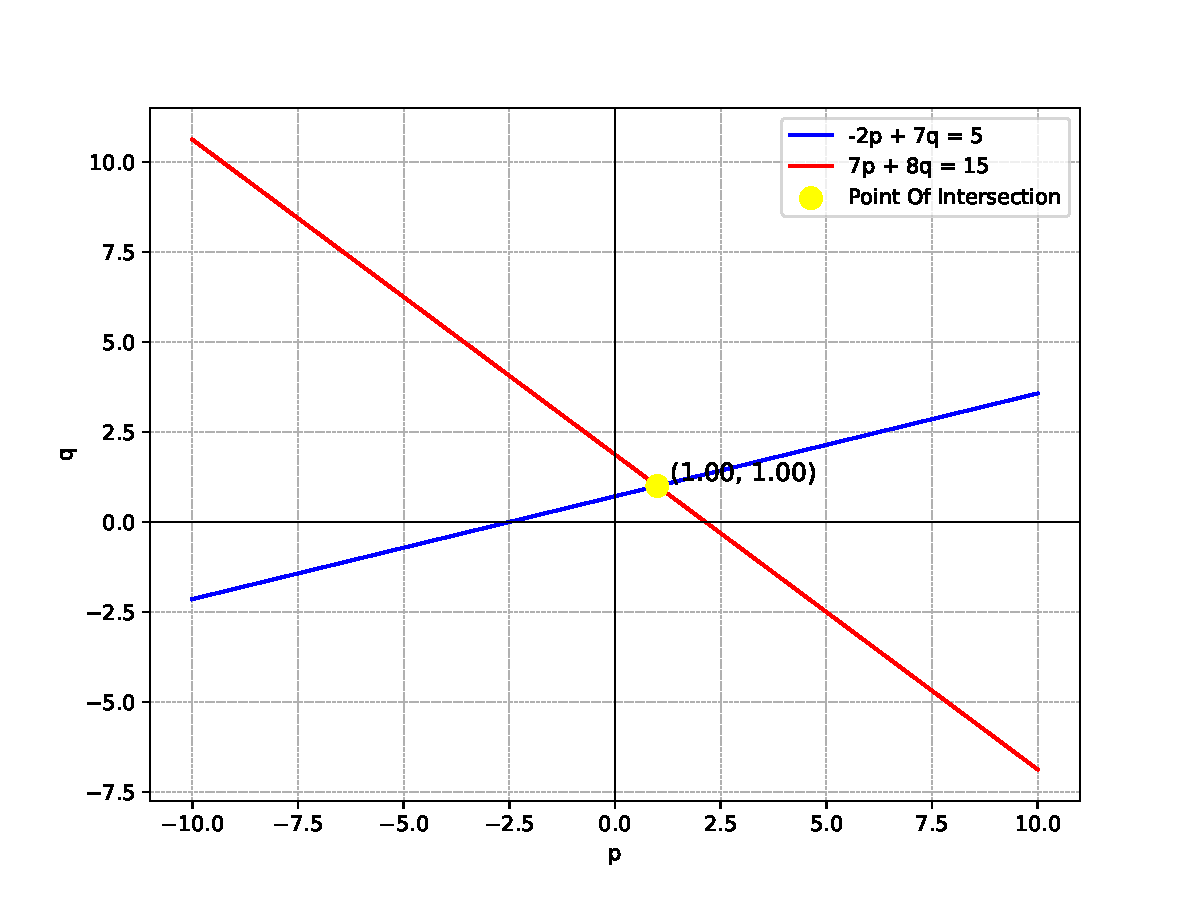
\includegraphics[width=\columnwidth]{figs/fig.pdf}
	\caption{Plot}
\end{figure}

\end{document}
